\documentclass[11pt]{article}
\usepackage[utf8]{inputenc} 
\usepackage{geometry}
\geometry{a4paper} 

%%% PACKAGES
\usepackage{subfig}
\usepackage{hyperref}
\usepackage{graphicx}

%%% HEADERS & FOOTERS
\usepackage{fancyhdr}
\pagestyle{fancy} 
\renewcommand{\headrulewidth}{0pt}
\lhead{}\chead{}\rhead{}
\lfoot{}\cfoot{\thepage}\rfoot{}

%%% SECTION TITLE APPEARANCE
\usepackage{sectsty}
\allsectionsfont{\sffamily\mdseries\upshape} 

%%% END Article customizations

%%% The "real" document content comes below...

\title{Schematisation in the Work of G.P. Shchedrovitsky}
\author{Marvin Müller\\[.3cm] Universität Leipzig -- Seminar Complex Systems
  and Co-operative Action }

\date{December 7, 2021}

\begin{document}
\maketitle

\section{Definition of terms}
\subsection{Methodology}
Methodology describes the theory of methods from a single discipline and the general theory of scientific methods as part of logic and philosophy \cite{2}. 

\subsection{Activity theory}
\begin{itemize}
	\setlength\itemsep{0em}
	\item naturalistic theory: world consists of human subjects and objects
	\item differs from this: objects are secondary constructs whose nature depends on the activity applied to them
	\item activity is a system that determines how individuals behave
	\item task of a scientist: examine objects in a specific scientific framework and choose a mothodology that marks a subject as a distinct subject of scientific enquiry (objects can be viewed from different perspectives) \cite{1}
\end{itemize}

\section{G.P. Shchedrovitsky}

\begin{itemize}
	\setlength\itemsep{0em}
	\item born in Moscow in 1929
	\item father was engineer in the Soviet aviation industry, mother microbiologist
	\item began to study at the Faculty of Philosophy of Moscow State University in 1949 and graduated 1953 with honors
	\item worked from 1951 to 1958 as a school teacher
	\item published his first scientific article in 1957
	\item began to develop seminars that attracted scientist from different disciplines who focused their discussions of logical and epistemological issues
	\item became part of the Moscow Methodological Circle and took the leadership in 1954
	\item developed the activity theory \cite{1}
\end{itemize}

\section{ Moscow Methodological Circle }
The specific approach of the MMC is that "systemic situations" are schematized in multi-position manner, which opens the prospect of collective problem solving as a multi-position organization of practices \cite[p. 270]{3}.
\\ \\
\noindent The basic concepts of the MMC can be formulated as four requirements to thinking:
\begin{enumerate}
	\item holism and reflexivity in relation to the other approaches and types of thinking (in science, design, engineering, socio-cultural and law studies, etc.)
	\item practical orientation (thinking-activity connections, which uses systems approach as the means for organizing processes of resolving complex problems by multi-professional and transdisciplinary teams, etc.)
	\item reflectivity as practical orientation of thinking to itself, i.e.  its capability to re-construct and re-direct itself
	\item the "methodological turn" from thinking about systems as objects to organizing, performing and reflecting the process of systems thinking in practice
\end{enumerate}
 

\section{Methodological School of Management}
With the Methodological School of Management V. B. Khristenko wants to give the reader the resources für self-organisation. It is a collection of techniques, methods of work and rules of self-organisation based on the work of G. P. Shchedrovitsky. The MSoM addresses organisers, leaders and managers \cite[p. 36]{5}. \\ 

\noindent Khristenko defines the act of activity as following: \\
"We obtain some source material, capture it and apply to it certain actions, tools or equipment, in order to transform it into a particular product, meeting a goal. This product emerges from the act of activity. We use tools and equipment." \cite[p. 36]{5} \\
Activities can be different from different perspectives. Is an excavator operator digging a ditch or operating the excavator? Khristenko states that when someone has learned how to operate the machine then he or she is digging a ditch. \\

\begin{figure}[h] 
  \centering
     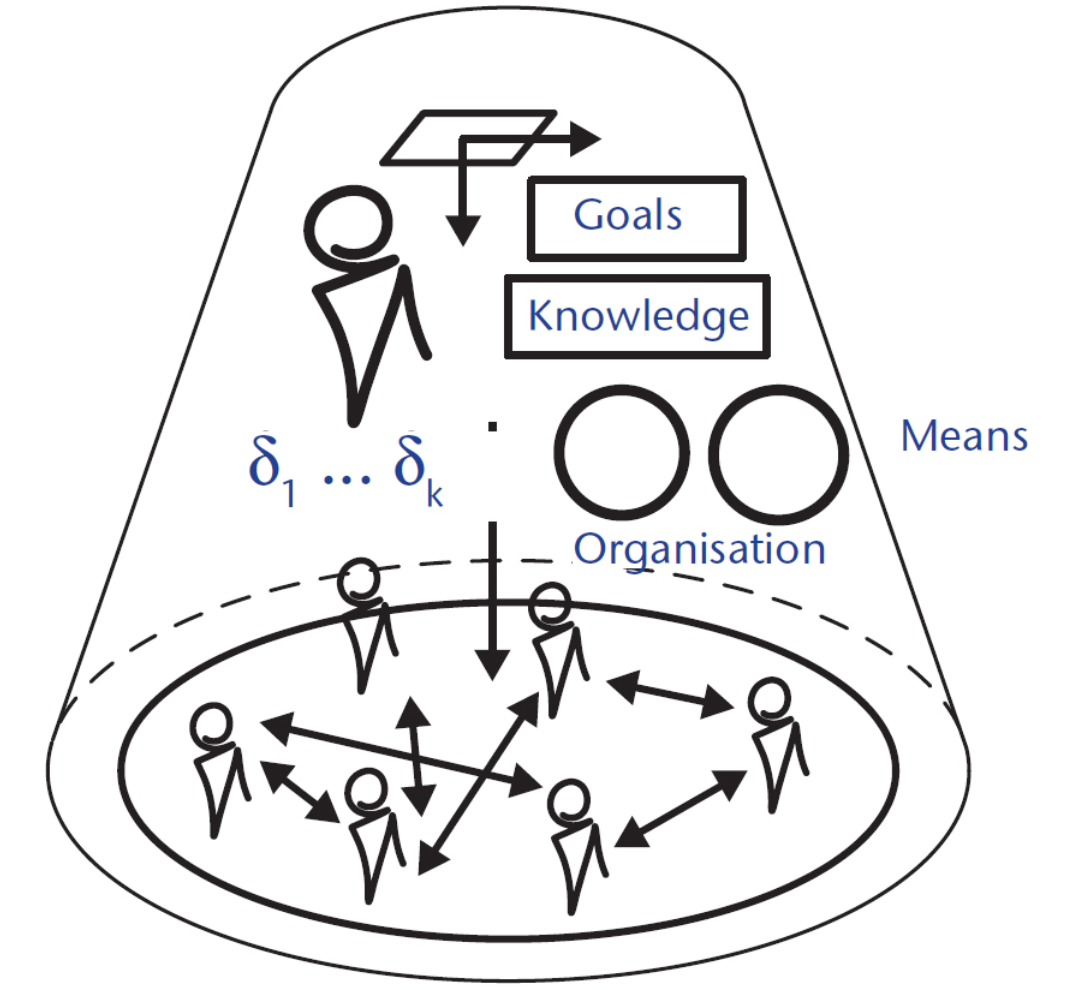
\includegraphics[width=200px]{fig1.png}
  \caption{Activity relations with a leading person \cite[p. 38]{5}}
  \label{ARLP} 
\end{figure}

\noindent Activities can also be related. For example, when someone’s work produces a product which is the source material for another person. The product can either be tools, equipment, or knowledge.
The product of a leading person may not be a transformation of natural material but can organize the activity of other people. The leader can influence other activities by changing goals, giving other knowledge and source material or by introducing new technology \cite[p. 38]{5}. How these changes effect the other activities and how changes should be made to come to a desired result is examined in Organizational-activity Games proposed by Shchedrovitsky.


\section{Organizational-activity Games by Shchedrovitsky}
OAGs are development games, as opposed to brainstorms or role-playing games usually aimed at handling certain concrete problems or situations \cite{4}.  

\subsection{Initial Phase}
\begin{itemize}
	\setlength\itemsep{0em}
	\item	 basis is a problem that cannot be resolved with current potential 
	\item participants should be from different fields of science (mostly problems involve several disciplines)
	\item not just theoreticians but also organizers, engineers, developers etc. should \\ participate
	\item the team should also include methodologists and game technicians
	\item game rule: if you suggest something you have to do it yourself
\end{itemize}

\subsection{Phase 1}
This is the phase of the participants’ self-determination, setting their own goal towards the "big" problem circumstances and "small" circumstances of the game itself. 
\begin{itemize}
	\setlength\itemsep{0em}
	\item	check and exchange knowledge and work methods
	\item first result: problem circumstances in new perspective, feel tense relations
	\item everyone formulates three objectives: professional, game and work related
	\item understanding that there is a gap between resources at hand and the objectives set 
\end{itemize}

\subsection{Phase 2}
\begin{itemize}
	\setlength\itemsep{0em}
	\item	integration between methodologists and professional experts
	\item OAG is based not on the right answer but on the correct formulation of the problem (it should demonstrate what exactly we need to solve the problem)
\end{itemize}

\subsection{Phase 3}
\begin{itemize}
	\setlength\itemsep{0em}
	\item	 adopt results to a "big" situation
	\item find a balance between mind, claim, and deed
\end{itemize}

\subsection{Khristenko's experiences with OAGs}
The first OAG Khristenko participated in took place in the year 1988 when he was the junior manager at the Chelyabinsk Tractor Plant  \cite[p. 38 et seqq.]{5}. Two years before the Perestroika period started and industrial, economic and social infrastructures in the Soviet Union were breaking down. As many others Khristenko saw his chance to be part of the radical change and registered himself for the OAG which was called "The development of a region within the framework of the development of a town".\\
This OAG led to several suggestions the author proposed to the director of the tractor plant, e.g.:
\begin{itemize}
	\setlength\itemsep{0em}
	\item old-school methods (12-hour shifts, extra work shifts, shouting at staff) should be abolished
	\item the plant should be independent and allowed to keep the ownership of the manufactured products
	\item new organisation concept: production association, corporation, concern or a consortium
	\item move away from the idea of "production for the sake of production" to an idea that we need to meet the demands created by a marketing system
\end{itemize}
According to Khristenko thanks to the OAG "these ideas had been well thought out, well put together and well formulated". After that he participated in many other OAGs during the Perestroika period e.g.
\begin{itemize}
	\setlength\itemsep{0em}
	\item "Ways of developing and raising the efficiency of the servicing of Kamaz Trucks for the national economy" (11 - 18 November 1988)
	\item "Prospects and programmes for the development of automobile manufacturing in the USSR" (16 - 24 December 1989)
	\item "A programme for the regional development of the city of Chelyabinsk and the Chelyabinsk Region" (26 November–3 December 1990)
\end{itemize}

	
\begin{thebibliography}{99}
 \bibitem{1} \url{en.wikipedia.org/wiki/Georgy_Shchedrovitsky}
 \bibitem{2} \url{https://www.ethnologie.uni-hamburg.de/pdfs-de/ethnoscripts-pdf/es10_2_artikel.pdf}
 \bibitem{3} Maracha, Viacheslav. (2018). Systems Thinking and Collective Problem Solving Practices. 269-272. 10.33278/SAE-2018.eng.269-272. 
 \bibitem{4} Naumov, S. B., Organizational-activity Games, Nature (Priroda), vol. 4, 1987.
 \bibitem{5} Khristenko, V. B., et al. Methodological School of Management, Bloomsbury Publishing Plc, 2014. ProQuest Ebook Central.
\end{thebibliography}


\end{document}
